\documentclass{jsarticle}
\oddsidemargin=-0.8cm
\topmargin=-2cm
\baselineskip=13pt
\textheight=55\baselineskip
\marginparsep=0.5in
\marginparwidth=0.5in
\textwidth=52zw
\usepackage{ascmac}
\usepackage{url}
\usepackage[dvipdfmx]{graphicx}
\usepackage[dvipdfmx]{color}
\usepackage{amsmath}
\usepackage{amssymb}
\usepackage{multicol}
\usepackage{bm}
\usepackage{here}
\usepackage{enumerate}
\usepackage{listings}
\usepackage{fancybox}
\usepackage{framed}
\usepackage{subfigure}
\usepackage{ccaption}
\usepackage{color}
\makeatletter
\lstset{% 
language={C}, 
frame=trbl,% 
basicstyle={\small},% 
identifierstyle={\small},% 
commentstyle={\small\ttfamily},% 
keywordstyle={\small\bfseries},% 
ndkeywordstyle={\small},% 
stringstyle={\small\ttfamily}, 
tabsize=2,
breaklines=true, 
frame=none,
columns=[l]{fullflexible},% 
numbers=left,% 
xrightmargin=0zw,% 
xleftmargin=3zw,% 
numberstyle={\scriptsize},% 
stepnumber=1, 
numbersep=1zw,% 
backgroundcolor={\color[gray]{.90}},
} 
\makeatother

\newenvironment{problems}
{
  \renewcommand\labelenumi{\doublebox{\arabic{enumi}}}
  \begin{enumerate}
}{
  \end{enumerate}
  \renewcommand\labelenumi{\arabic{enumi}.}
}

\pagestyle{empty}	

\begin{document}
\title{基礎気象学講義 復習問題} % ここは毎回同じ
\author{第6回} %authorの代わりに第何回かを入れる
\date{雲と降水の分類} %内容を記載する
\maketitle

\section{問題}

    \begin{problems}
    \item 次の問いに答えなさい。
        \begin{enumerate}[(1)]
        \item 雲は大きく10種類に分かれる(十種雲形)。これらを出る層がわかるように一覧に並べ、和名・英名・記号をまとめた表を作成しなさい。
        \item 気象観測の手引き(\url{https://www.jma.go.jp/jma/kishou/know/kansoku_guide/tebiki.pdf})に従い、次の降水現象を説明しなさい。
        \begin{itemize}
            \item 霧雨
            \item 着氷性・過冷却の霧雨
            \item 雨
            \item 着氷性・過冷却の雨
            \item 雪
            \item みぞれ
            \item 雪あられ
            \item 霧雪
            \item 凍雨
            \item 氷あられ
            \item ひょう
            \item 細氷\\
        \end{itemize}
        \end{enumerate}

    \item 昼間に空を観測し、全雲量・各層の雲の型・出ている雲形とその雲量・天気を記録しなさい。これを6時間以上あけて3度以上行うと共に、その時の空の写真を貼り付けなさい。\\

    \item International Cloud Atlas(国際雲図帳、\url{https://cloudatlas.wmo.int/en/home.html})のサイトには、WMO(世界気象機関)の提供する様々な雲に関する知見がまとめられている。
        当該サイトのImagesから適当な雲の写真を3点選び、その解説を和訳しなさい。

\end{problems}

\section{答案}
\begin{problems}
\item
% 以下に解答を作成してGit Push。
	\begin{enumerate}[(1)]
  \item 
  \begin{table}[H]
\begin{tabular}{|l|l|l|l|}
\hline
   & 和名  & 英名            & 記号 \\ \hline
   & 巻雲  & Cirrus        & Ci \\ \cline{2-4} 
上層 & 巻積雲 & Cirrocumlus   & Cc \\ \cline{2-4} 
   & 巻層雲 & Cirrostratus  & Cs \\ \hline
   & 高積雲 & Altocumulus   & Ac \\ \cline{2-4} 
中層 & 高層雲 & Altostratus   & As \\ \cline{2-4} 
   & 乱層雲 & Nimbostratus  & Ns \\ \hline
   & 層積雲 & Stratocumulus & Sc \\ \cline{2-4} 
下層 & 層雲  & Stratus       & St \\ \cline{2-4} 
   & 積雲  & Cumulus       & Cu \\ \cline{2-4} 
   & 積乱雲 & Cumulonimbus  & Cb \\ \hline
\end{tabular}
\end{table}

\item \begin{table}[H]
\begin{tabular}{|l|l|}
\hline
霧雨         & 直径0.5mm未満のきわめて多数の細かい水滴だけがかなり一様に降る降水                     \\ \hline
着氷性・過冷却の霧雨 & 0℃より低音の霧雨                                               \\ \hline
雨          & 水滴からなる降水のことである。 \\ \hline
着氷性・過冷却の雨  & 0℃より低音の雨                                                \\ \hline
雪          & 空気中の水蒸気が昇華してできた氷の結晶の降水                                  \\ \hline
みぞれ        & 雨と雪とが混在して降る降水                                           \\ \hline
雪あられ       & 白色で不透明な氷の粒の降水                                           \\ \hline
霧雪         & ごく小さい白色で不透明な氷の粒の降水                                      \\ \hline
凍雨         & 透明の氷の粒の降水                                               \\ \hline
氷あられ       & 半透明の氷の粒の降水                                              \\ \hline
ひょう        & 氷の小粒又はかたまりの降水                                           \\ \hline
細氷         & 晴れた空から降ってくるごく小さな氷の結晶の降水。大気中に浮遊しているように見える                \\ \hline
\end{tabular}
\end{table}
  \end{enumerate}
\item 

1枚目(2-1.png)\\
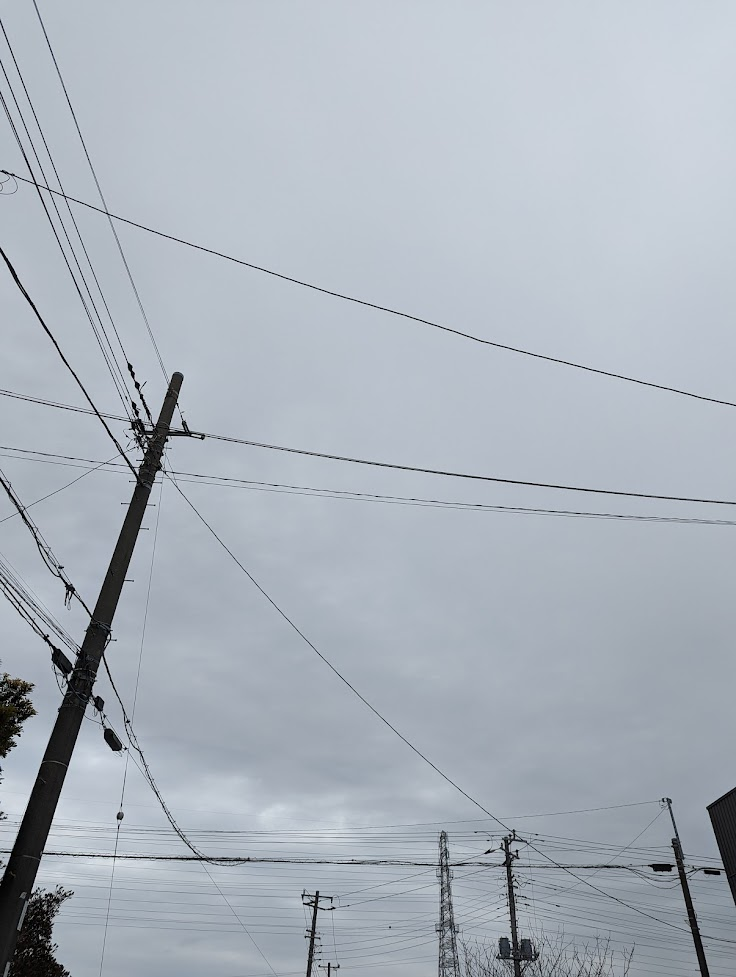
\includegraphics[width=7cm]{2-1.png}\\

2- Sc x x\\
8+ As x x\\
2枚目(2-2.png)\\
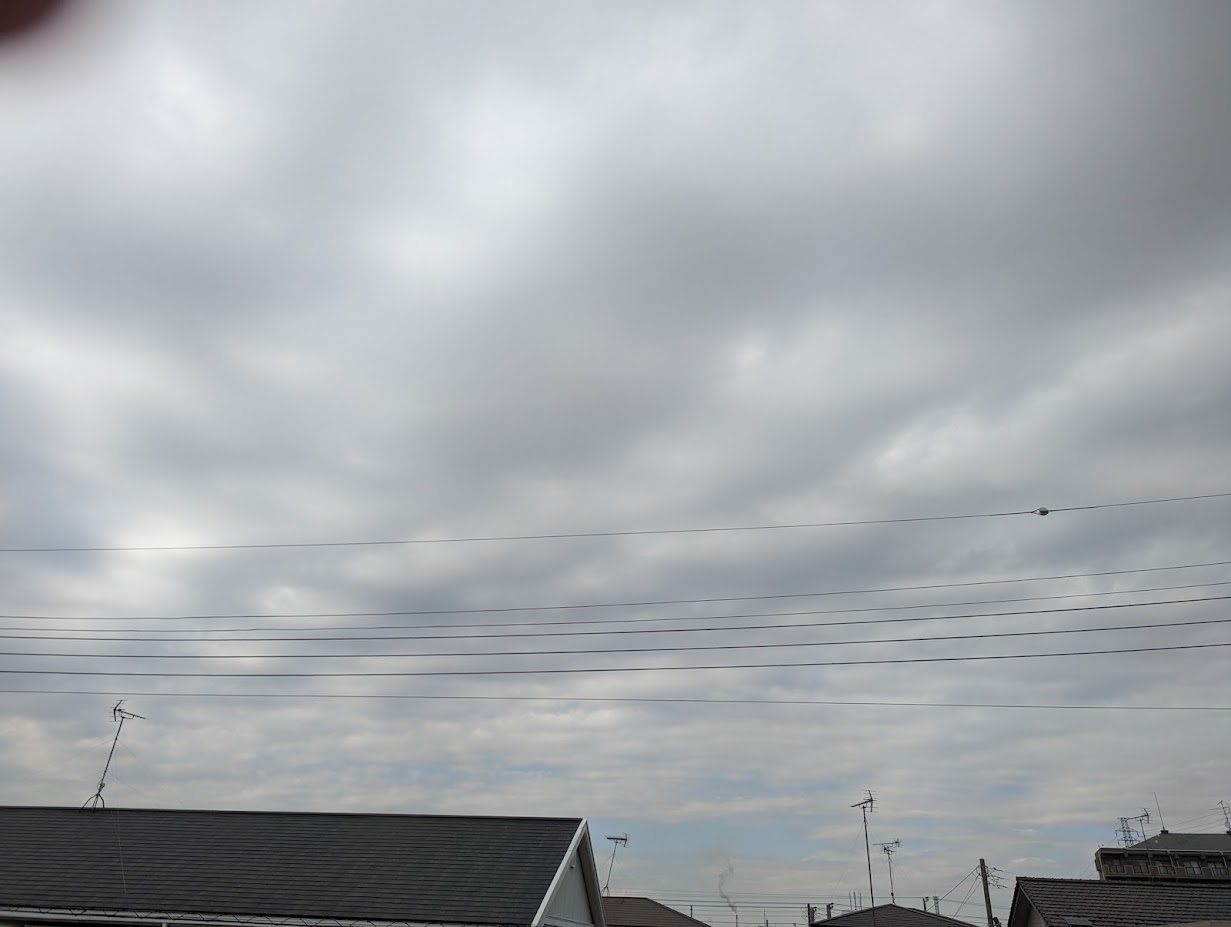
\includegraphics[width=7cm]{2-2.png}\\
9+ As x x\\


3枚目(2-3.png)\\
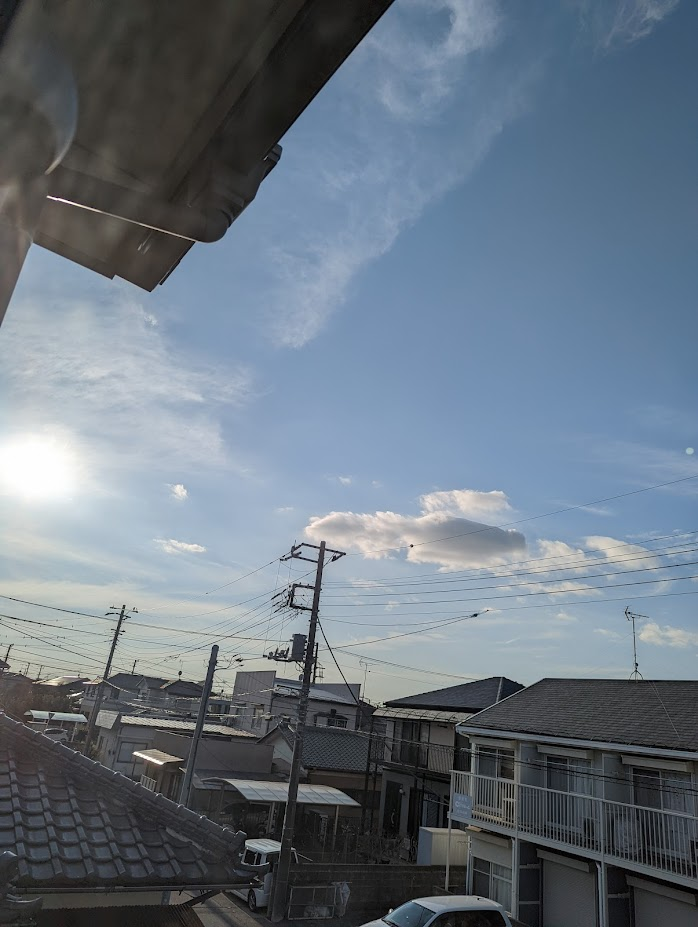
\includegraphics[width=7cm]{2-3.png}\\
1 Cu x x\\
3+ Ci x x\\

\item 
1枚目(3-1.png)\\
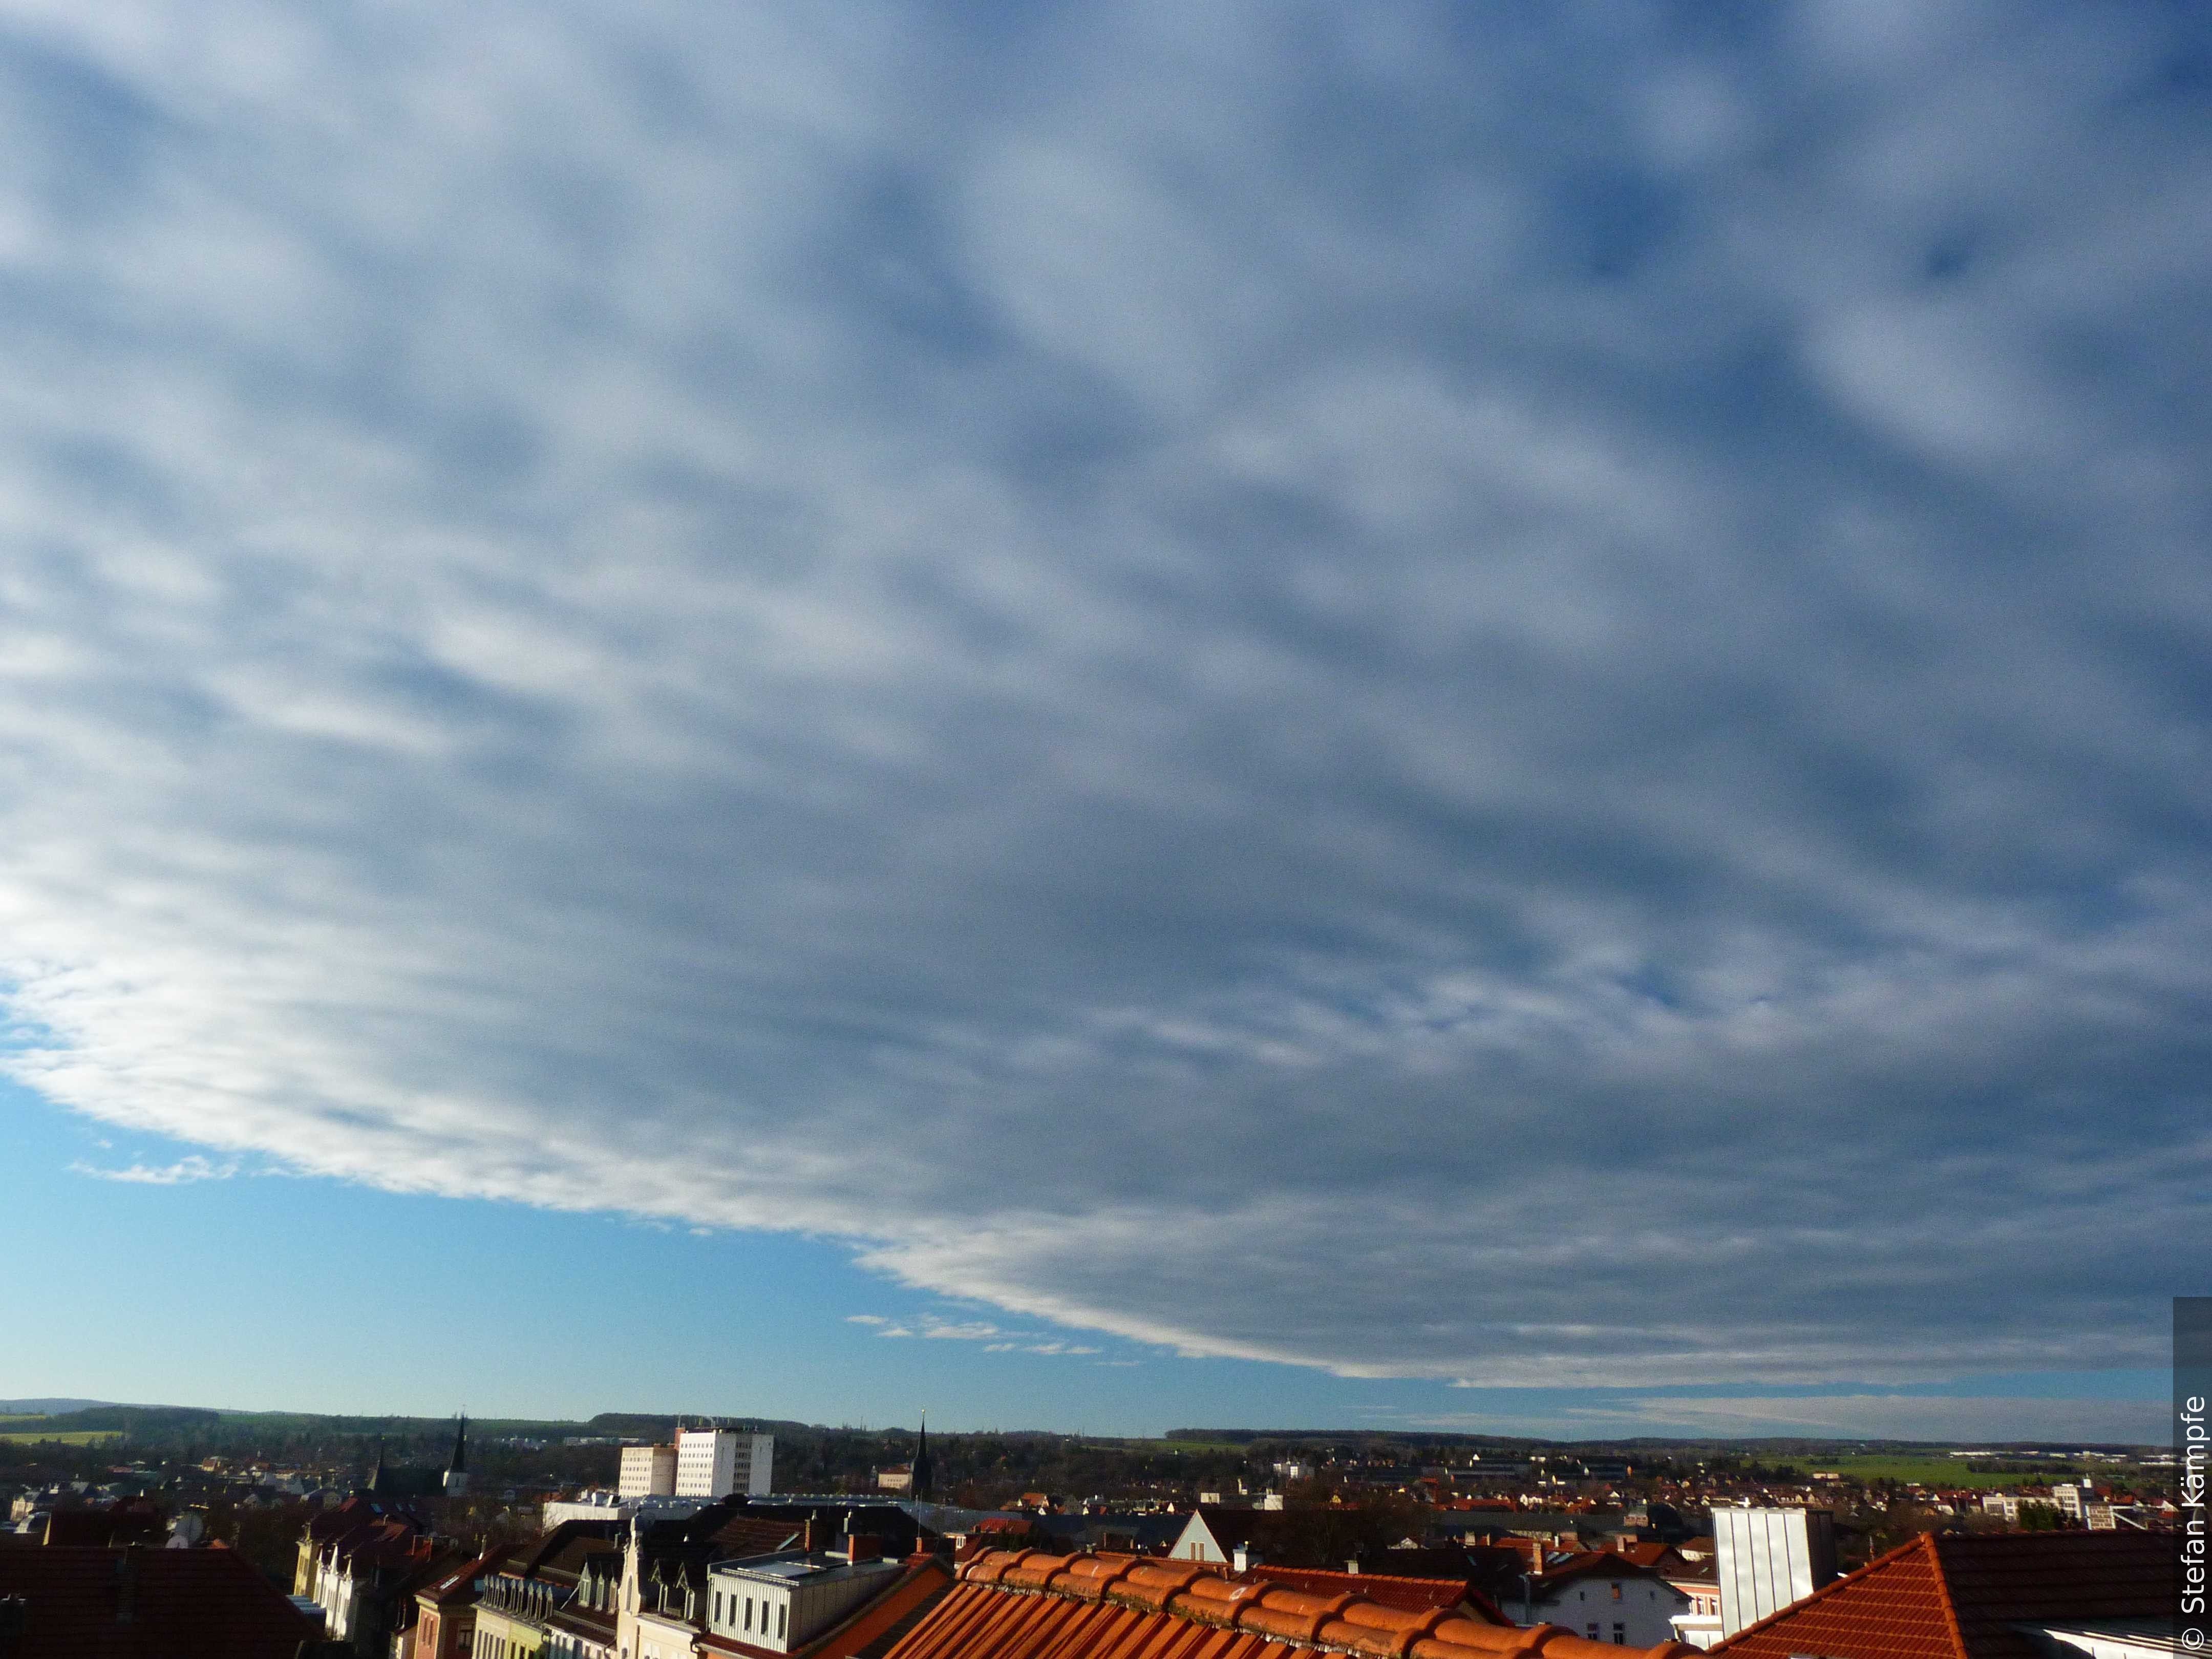
\includegraphics[width=7cm]{3-1.png}
This photograph shows a whitish to grey layer of Stratocumulus cloud that has some darker parts and displays the fairly flattened base associated with the species stratiformis. The layer is sufficiently thin or translucent that it could reveal the position of the Sun; this is the variety translucidus. In addition, there are spaces between the cloud elements, through which some blue sky can be seen at 2 and 3; this is the variety perlucidus.
\\英訳\\
この写真は、白〜グレーのScがあり、一部暗いところが見え、層状雲によく見られるほとんど平らであることも見られる。層が薄く、半透明なので、太陽の位置がわかる可能性がある。また、2,3に雲の隙間があり、そこから青空が見えている。
\\
2枚目(3-2.png)\\
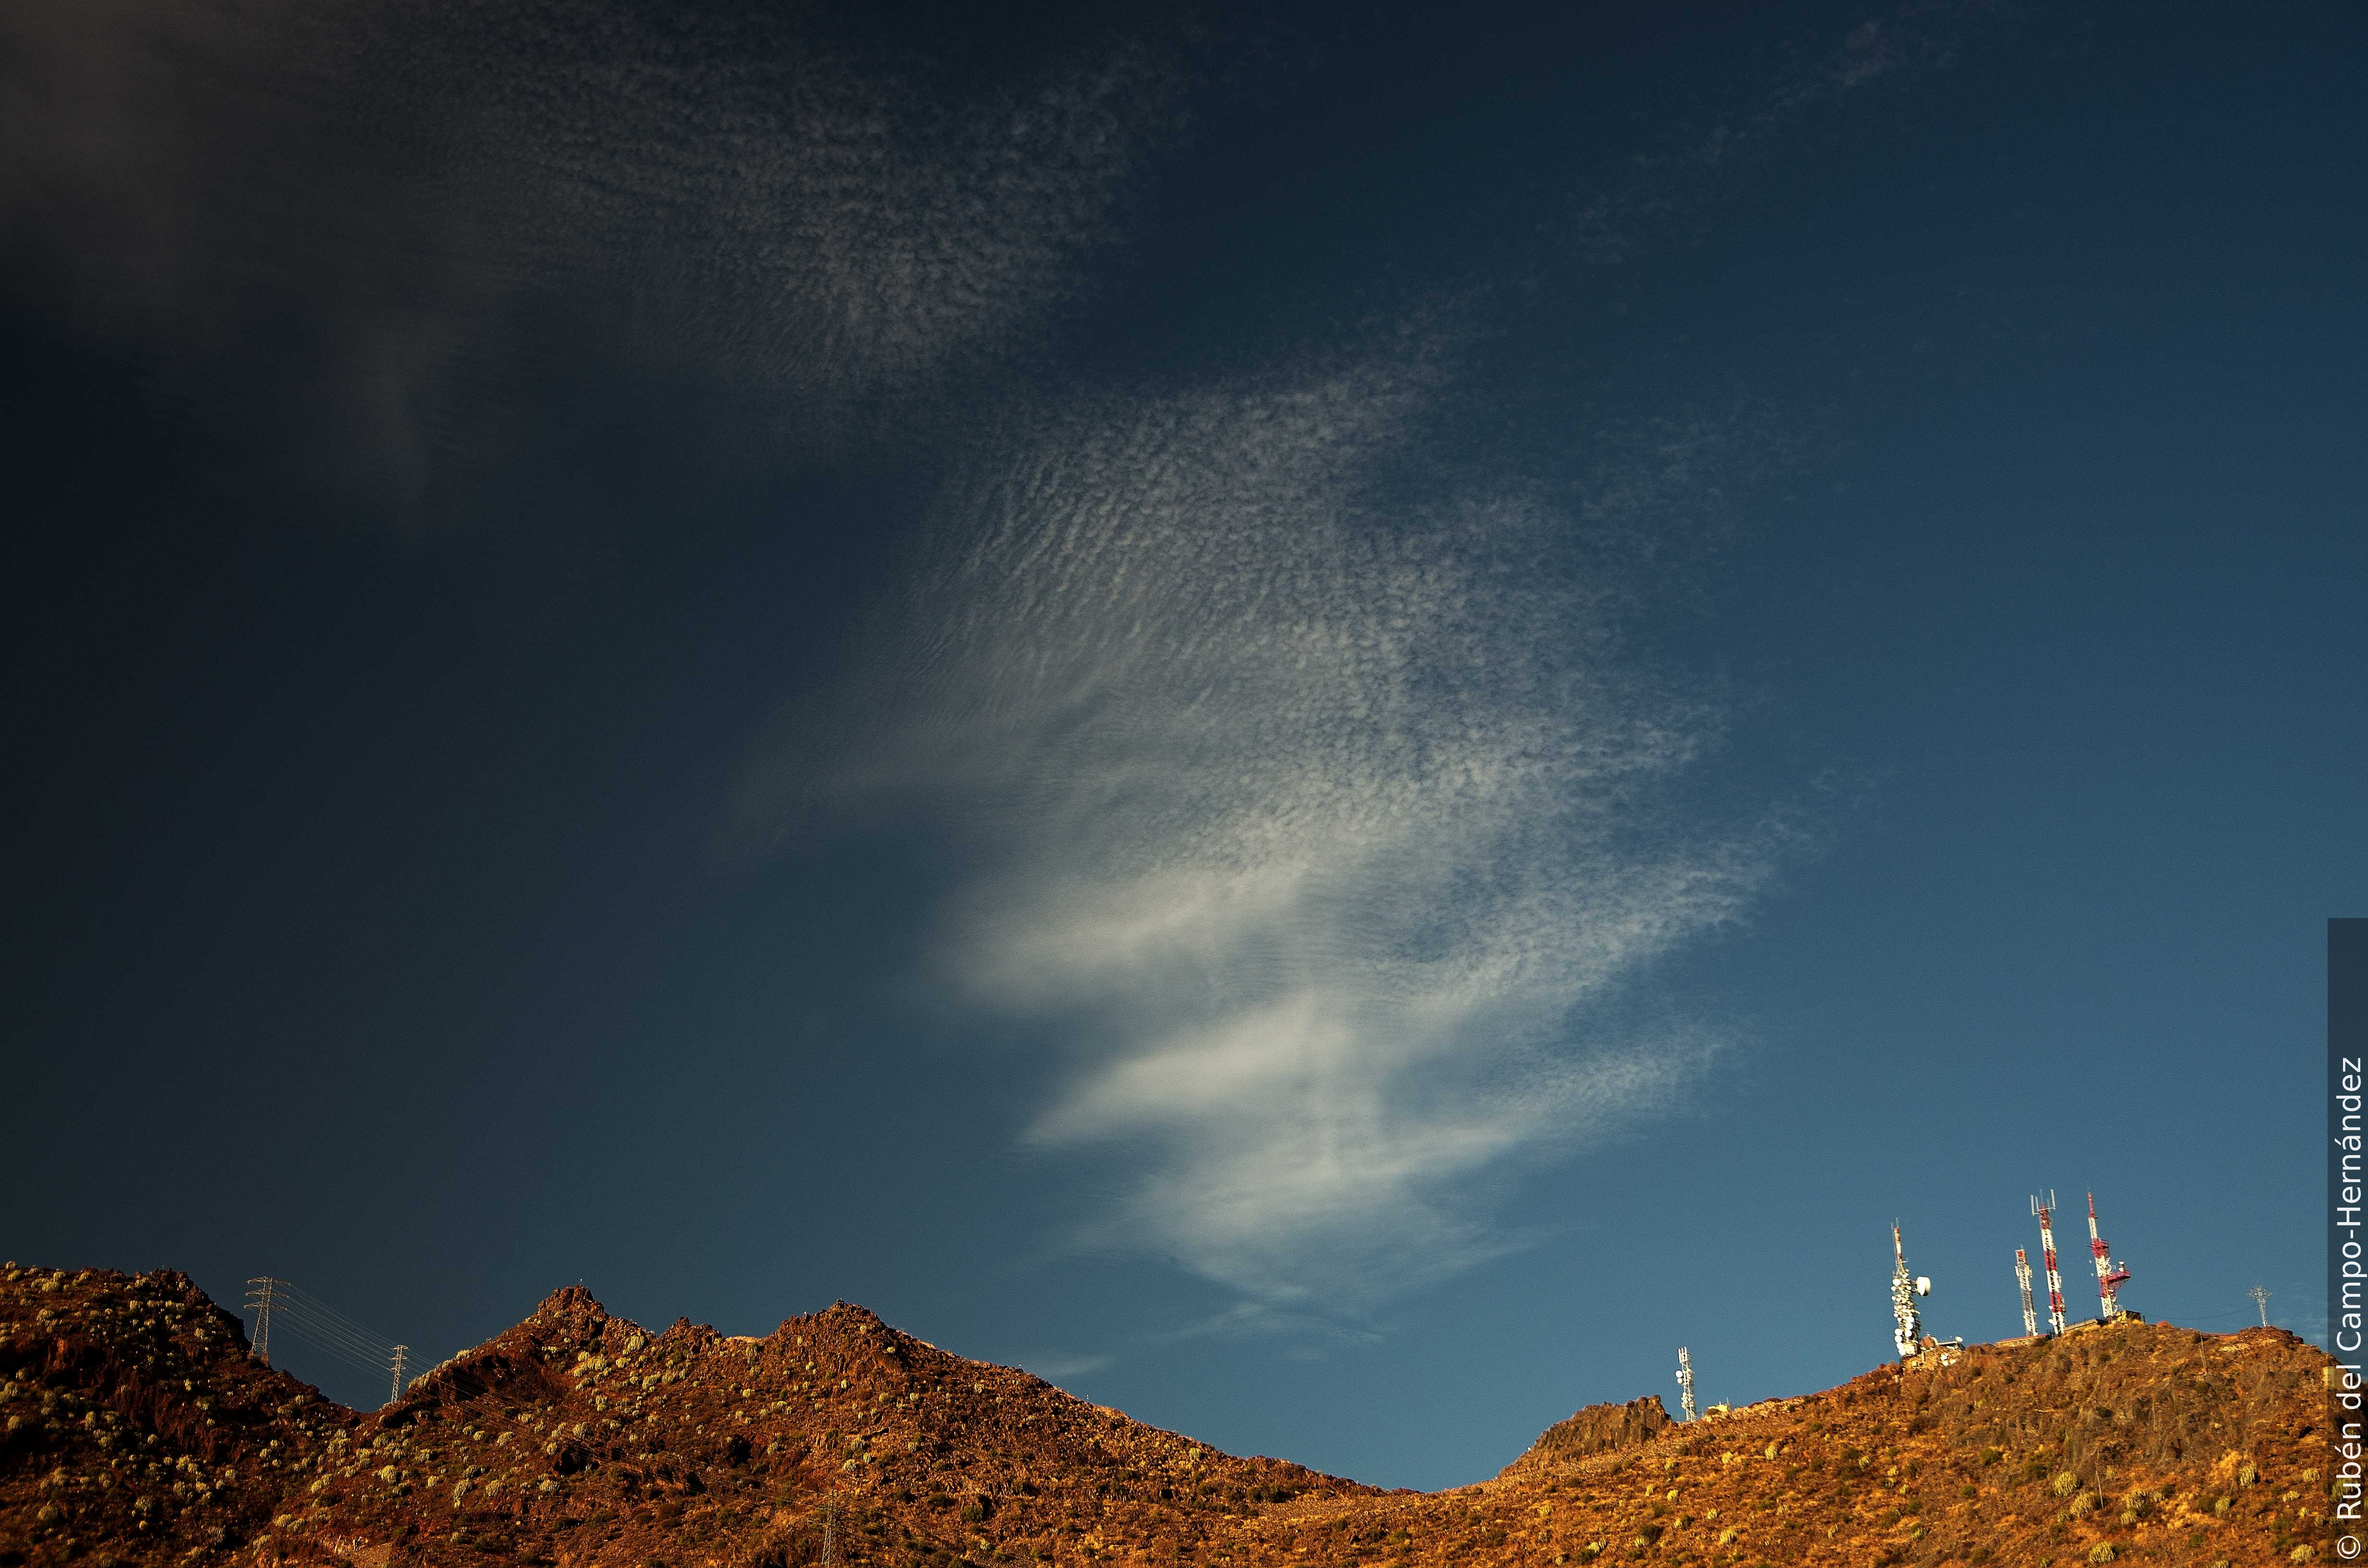
\includegraphics[width=7cm]{3-2.png}

Cirrocumulus usually appears as a patch of cloud as seen here, consisting of very small elements that are also called cloudlets. Both aspects are typical of the genera. The elements have an apparent width of less than 1° and are of the species floccus. The undulations indicate the variety undulatus and beneath the merged floccus are short trails of virga, which are a supplementary feature. Near the top of the image are what appear to be the hanging protuberances of the supplementary feature mamma. It should be noted that mamma at such a height in Cirrocumulus would be very small. 
\\英訳\\
Ccは通常、雲のパッチ?として現れ、雲粒と呼ばれる非常に小さい要素で構成されている。今回はどちらも含まれている。雲粒は幅が1°未満であり、種類はふさ状雲(flo)である。floの下に尾流雲(vir)があり、波状雲(un)も見られる。画像の上部に乳房雲(mam)が見られる。なお、この高さにあるCcに付属するmamは非常に小さい。
\end{problems}

3枚目(3-3.png)\\
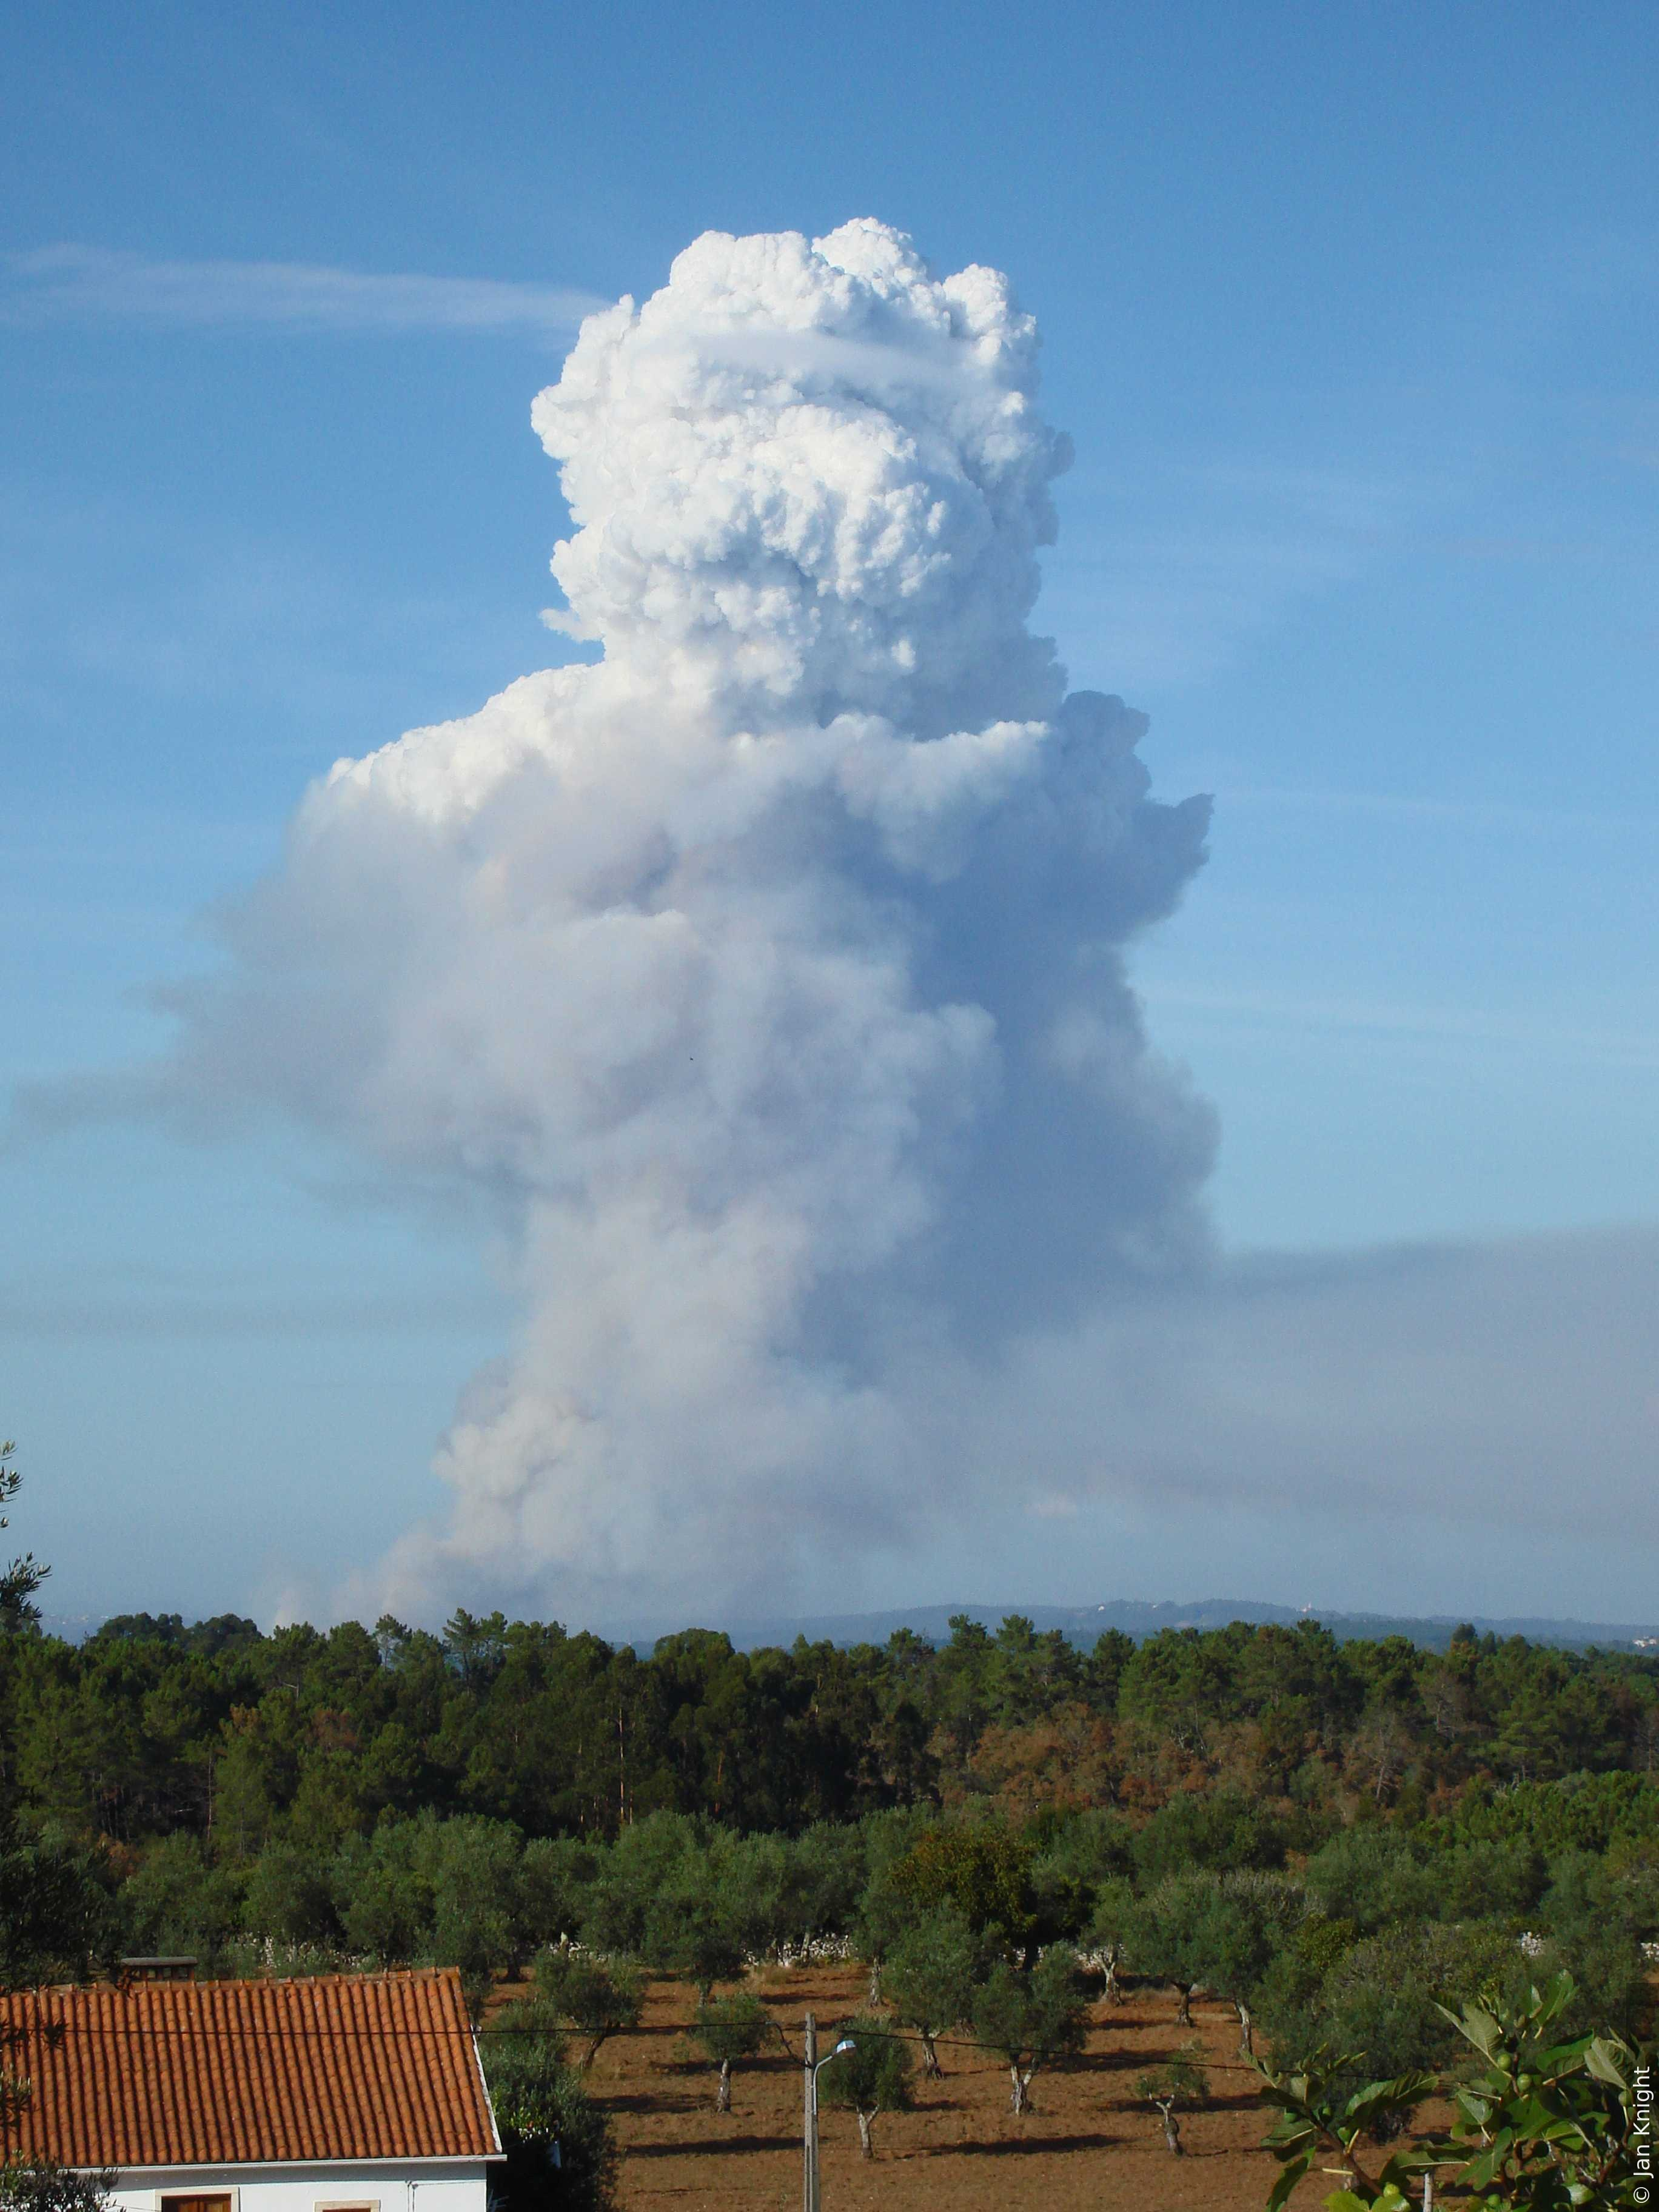
\includegraphics[width=7cm]{3-3.png}
This picture, taken from Serra de Alvorge in Portugal, shows a Cumulus congestus generated as a result of rising thermals from a wildfire. It is therefore classified as Cumulus congestus flammagenitus.

Light, north-westerly, low-level winds caused smoke from the wildfire to drift slowly to the south-east and some smoke also rose vertically into the lower atmosphere. However, the atmosphere was deeply unstable above about 2 300 m and the convective plume rose quickly to considerable height, resulting in the formation of a tower of Cumulus congestus flammagenitus.
\\英訳\\
この写真は、ポルトガルのセラ・デ・アルボルジで撮影されたもので、山火事による上昇気流によって発生したCbである。そのため、Cumulus congestus flammagenitusと分類されている。北西の弱い風により、山火事の煙が南東に流れて、大気圏下層に鉛直に上昇した。しかし、高度2300m超えたあたり大気圏は不安定なので、煙は急速に上層したため、Cumulus congestus flammagenitusの雲が発生した。
\end{document}

